\documentclass[paper=letter, fontsize=14pt]{scrartcl} 


\usepackage[utf8]{inputenc}
\usepackage{color}
\usepackage{hyperref}
\usepackage{graphicx}
\usepackage{epsfig}
\usepackage{multirow}
\usepackage{colortbl}
\usepackage[table]{xcolor}
\usepackage{fancyhdr}
\usepackage{graphicx}
\usepackage{graphicx}
\usepackage{verbatim}
\usepackage{pictex}  
\usepackage{multimedia}
\usepackage{listings}
\usepackage{vmargin}
\usepackage{xcolor,colortbl}
\usepackage[spanish]{babel} % language/hyphenation
\usepackage{amsmath,amsfonts,amsthm} % Math packages
\usepackage{amsbsy}
\usepackage{amssymb}
\usepackage{fancyvrb}
\usepackage{sectsty} % Allows customizing section commands
\allsectionsfont{\centering \normalfont\scshape} % Make all sections centered, the default font and small caps

\usepackage{fancyhdr} % Custom headers and footers
\pagestyle{fancyplain} % Makes all pages in the document conform to the custom headers and footers
\fancyhead{} % No page header - if you want one, create it in the same way as the footers below
\fancyfoot[L]{} % Empty left footer
\fancyfoot[C]{} % Empty center footer
\fancyfoot[R]{\thepage} % Page numbering for right footer
\renewcommand{\headrulewidth}{0pt} % Remove header underlines
\renewcommand{\footrulewidth}{0pt} % Remove footer underlines
\setlength{\headheight}{13.6pt} % Customize the height of the header

\numberwithin{equation}{section} % Number equations within sections (i.e. 1.1, 1.2, 2.1, 2.2 instead of 1, 2, 3, 4)
\numberwithin{figure}{section} % Number figures within sections (i.e. 1.1, 1.2, 2.1, 2.2 instead of 1, 2, 3, 4)
\numberwithin{table}{section} % Number tables within sections (i.e. 1.1, 1.2, 2.1, 2.2 instead of 1, 2, 3, 4)
\setpapersize{A4}
\setmargins{2.5cm}       % margen izquierdo
{2.4cm}                        % margen superior
{16.5cm}                      % anchura del texto
{23.42cm}                    % altura del texto
{10pt}                           % altura de los encabezados
{1cm}                           % espacio entre el texto y los encabezados
{0pt}                             % altura del pie de página
{2cm}                           % espacio entre el texto y el pie de página

\setlength\parindent{0pt} % Removes all indentation from paragraphs - comment this line for an assignment with lots of text

\newcommand{\horrule}[1]{\rule{\linewidth}{#1}} % Create horizontal rule command with 1 argument of height

\title{	
\normalfont \normalsize 
\textsc{Centro de Investigaci\'on en Matem\'aticas (CIMAT). Unidad Monterrey} 
\\ [25pt] 
\horrule{0.5pt} \\[0.4cm] % Thin top horizontal rule
\huge \textbf{Densidad de ensembles y separaciones}\\ 
\horrule{2pt} \\[0.5cm] % Thick bottom horizontal rule
}

\author{Ricardo Cruz} % Your name

\date{\normalsize\today} % Today's date or a custom date


\rhead{\begin{picture}(0,0) \put(-56.7,-50){
\includegraphics[width=20mm]{cimat.png}} \end{picture}}
\renewcommand{\headrulewidth}{0.5pt}

\pagestyle{fancy}

\begin{document}
\lstdefinestyle{customc}{
  belowcaptionskip=1\baselineskip,
  basicstyle=\footnotesize, 
  frame=lrtb,
  breaklines=true,
  %frame=L,
  %xleftmargin=\parindent,
  language=C,
  showstringspaces=false,
  basicstyle=\footnotesize\ttfamily,
  keywordstyle=\bfseries\color{green!40!black},
  commentstyle=\itshape\color{red!40!black},
  identifierstyle=\color{blue},
  stringstyle=\color{purple},
}

\lstset{breakatwhitespace=true,
  basicstyle=\footnotesize, 
  commentstyle=\color{green},
  keywordstyle=\color{blue},
  stringstyle=\color{purple},
  language=C++,
  columns=fullflexible,
  keepspaces=true,
  breaklines=true,
  tabsize=3, 
  showstringspaces=false,
  extendedchars=true}

\lstset{ %
  language=R,    
  basicstyle=\footnotesize, 
  numbers=left,             
  numberstyle=\tiny\color{gray}, 
  stepnumber=1,              
  numbersep=5pt,             
  backgroundcolor=\color{white},
  showspaces=false,             
  showstringspaces=false,       
  showtabs=false,               
  frame=single,                 
  rulecolor=\color{black},      
  tabsize=2,                  
  captionpos=b,               
  breaklines=true,            
  breakatwhitespace=false,    
  title=\lstname,             
  keywordstyle=\color{blue},  
  commentstyle=\color{dkgreen},
  stringstyle=\color{mauve},   
  escapeinside={\%*}{*)},      
  morekeywords={*,...}         
} 


\maketitle % Print the title


\pagebreak


Al modelar un evento sumamente complejo, se opta por ocupar las matrices aleatorias y calcular promedios para inferir las propiedades estadísticas de la matriz original.\\

En la teoría de matrices aleatorias, existen tres tipos de matrices que poseen propiedades interesantes para desarrollar el proceso mencionado anteriormente, estos 3 tipos se resumen en los siguientes ensembles.

\begin{itemize}
\item GOE: Gaussian Orthogonal Ensemble, el cual es una matriz con entradas aleatorias y se simetriza mediante $(H+H')/2$
\item GUE: Gaussian Unitary Ensemble, es aquel que considera una matriz Hermitiana con entradas aleatorias y posteriormente lo simetriza.
\item GSE Gaussian Simplectic Ensemble, es el ensemble que considera como matriz aleatoria a una matriz simplectica.
\end{itemize}

La matriz de varianzas y covarianzas (matriz simétrica) contiene la información para deducir los valores propios y dependiendo de que ensemble ocupado, la distribución marginal de un valor propio puede variar.\\

En general la ley del semicirculo de Wigner se asemeja bastante a las densidades propuestas generadas por los distintos ensembles\\

La figura 1 y 2 muestra la densidad propuesta por Wigner y cada uno de las densidades generadas por los ensembles y diferentes tamaños de la matriz, a saber, 10 y 100


\begin{figure}[h]
  \centering
  \begin{minipage}[b]{0.47\textwidth}
    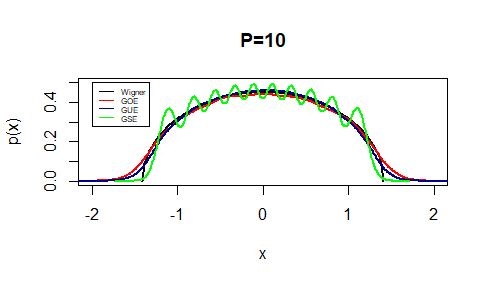
\includegraphics[width=\textwidth]{i1.png}
    \caption{p=10.}
  \end{minipage}
  \hfill
  \begin{minipage}[b]{0.47\textwidth}
    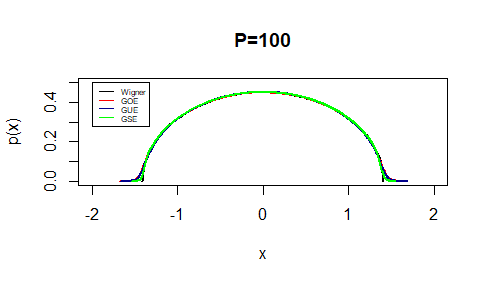
\includegraphics[width=\textwidth]{i2.png}
    \caption{p=100.}
  \end{minipage}
\end{figure}

Se puede apreciar que el comportamiento de la densidad se aproxima o asemeja más al semicirculo de Wigner en la segunda figura, por lo que se puede pensar que a medida que $p$ crece la densidad es igual a la ley de Wigner.\\

También es de interés conocer la distancia que existe entre los valores propios, pues presenta un comportamiento en el cual se aprecia la separación a la que tienden dos valores propios contiguos.\\

La figura 2 muestra la distancia de los eigenvalores a través de simulaciones monte carlo, además de compararlo con la distribución teórica que deberían seguir, deducida para $p=2$. En color rojo se muestra la simulación para $p=2$ y en color morado las simulaciones correspondientes a $p=100$. Se puede observar que a medida que $p$ crece la distribución simulada no se parece tanto a los valores teóricos y tiende a concentrarse en un punto cercano a 0.

\begin{figure}[h]
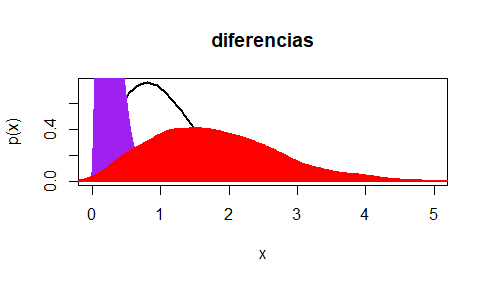
\includegraphics[scale=1]{i3.png} 
\caption{Distribución de las separaciones contiguas.}
\end{figure}

Los códigos se pueden encontrar en el repositorio asociado a la siguiente dirección: \url{https://github.com/Ricardo27cruz27/Matrices-aleatorias}

\pagebreak

\textbf{Las propiedades estadísticas del transporte en Cuernavaca y los ensembles de matrices aleatorias.}\\

Muchos fenómenos de la vida real son descritos a través de sistemas cuya complejidad es demasiada alta y en consecuencia el estudio de ellos, de manera directa, es una tarea que necesita de muchos recursos.\\

El constante avance tecnológico de los últimos años, ha permitido que la simulación realicé de manera más sencillas los procesos que antes eran imposibles o difíciles.\\

En este caso, el transporte de la ciudad de Cuernavaca, Morelos, puede verse como un sistema en el que varias entidades interactuan y cada una de ellas busca un beneficio propio. Este sistema se puede modelar con una ensemble gaussiano unitario (GUE).\\

En general este proceso se basa en un grupo de observaciones en las que se indica cual es el momento en que llega un autobus a la parada. La información se recolecto durante 27 días y cobra relevancia al poder modelar el tiempo que pasa entre la llegada de un autobus y otro, pues desde el punto de vista del conductor, dependiendo de este tiempo las personas a las que les pueda dar servicio dependerán de cuanto tiempo ha pasado desde el último autobus en esa estación. Desde la perspectiva social, se crearía un servicio eficiente en el cual se satisfaga de manera correcta las necesidades de la población.\\

Los resultados arrojados por el GUE en este modelo se adecuan de manera casi perfecta a los datos recolectados para las llegadas de los autobuses. Es decir, la separación entre los autobuses sigue una distribución semejante a la de la separación de los valores propios generados por el ensemble.\\

Así como este sistema, existen muchos fenómenos en la actualidad que podrían ser modelados por los teoría de matrices aleatorias, pues la misma naturaleza de las entidades involucradas se comportan como lo hacen los valores propios de los ensembles.



\end{document}
